\section{HERM-Schema}
\begin{figure}[ht]
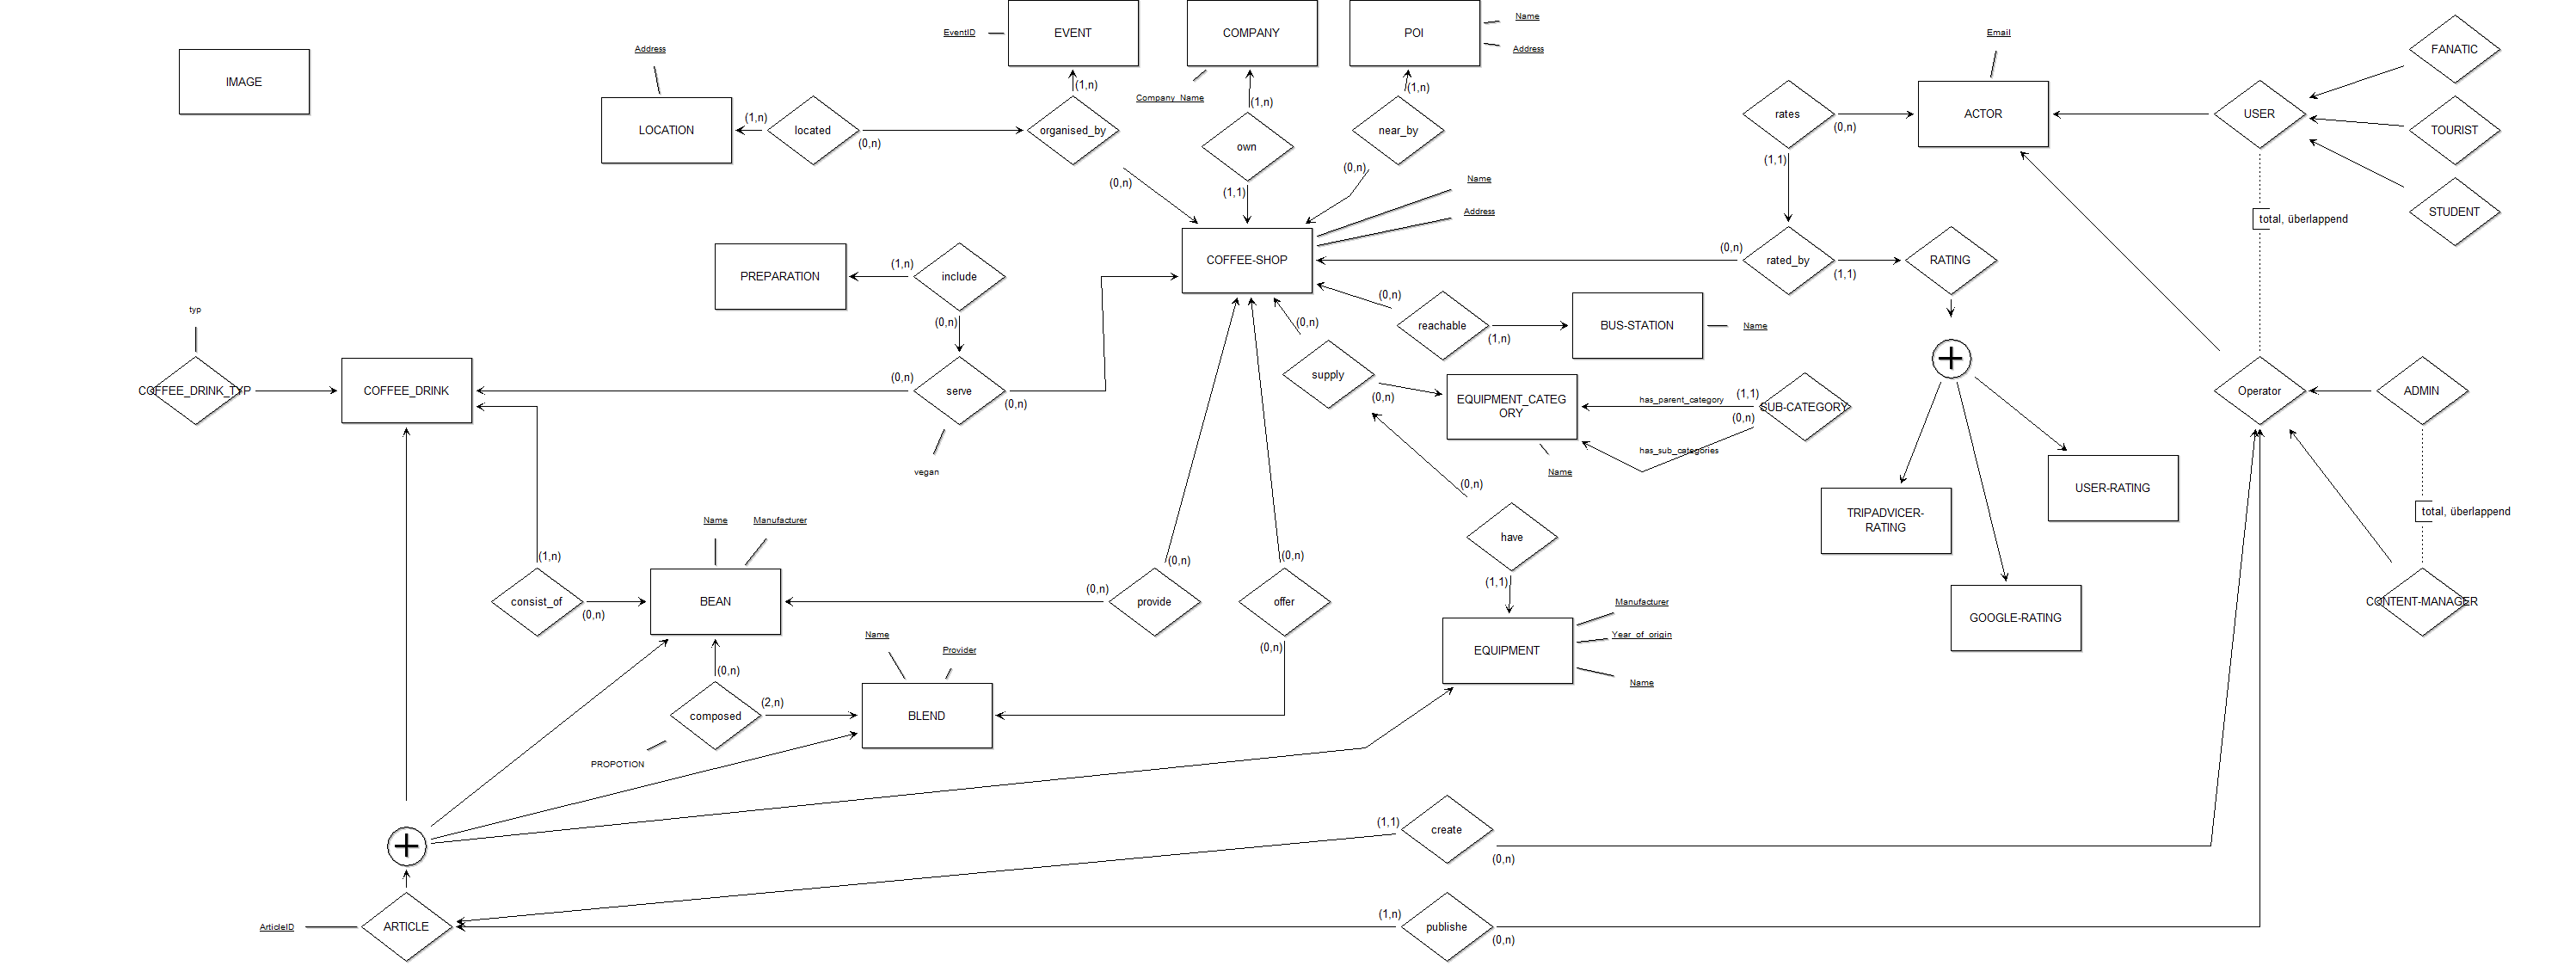
\includegraphics[
    page=1,
    width=\textwidth,
    height=\textheight,
    keepaspectratio
]{Content/HERM/Herm_coffee16_05.png}
\vfill
\caption{Simplify domain model}
\end{figure}
\subsection{HERM-Translation}
\subsubsection{Descripition}
Higher-Order\\
Located was translate by taken the primary key  of LOCATION aswell as the primary keys from the relationship of organised\_by.\\
Rated\_By was translated by\\
Includes was translate by taken the primary key of PREPARATION aswell as the primary keys from the relationship of serves.\\
Sells was translated by taken the primary key of EQUIPMENT aswell as the primary keys from the relationship supplies.\\\\ 
Cluster are transform with the full key approach, because the entities have no common keys in their entities. \\ 
The ARTICLE cluster with the connection to the following entites: EQUIPMENT, COFFEE\_DRINK, BEAN and BLEND.\\
The RATING cluster with the connection to the following entities: GOOGLE-RATING, USER-RATING, TRIPADVISER-RATING.\\\\
\subsubsection{Entity}
(EQUIPMENT(Manufacturer, Year\_of\_origin, Name)\\(Manufacturer, Year\_of\_origin, Name))\\
(EVENT(EventID, Time, Name,Access\_fee, Description)(EventID))\\
(COFFEE-SHOP(Name, Address, Outdoor, Fair\_trade, Disabled\_friendly, Description, Wlan, Child\_friendly, Website, Fouding\_year, Pet\_friendly, Latte\_art, Seats, Workstation, Food, Price\_class, Franchise)(Name, Address))\\
(BUS-STATION(Name, Line)(Name, Line))\\
(COMPANY(Name)(Name))\\
(BEAN(Name, Manufacturer, Provenance,Fair\_trade, Type)\\(Name, Manufacturer))\\
(POI(Name, Address, Description)(Name, Address))\\
(GOOGLE-RATING()())\\
(USER-RATING()())\\
(TRIPADVICER-RATING()())\\
(BLEND(Name, Manufacturer, Provenance, Price\_range)(Name, Manufacturer))\\
(LOCATION(Address, Description)(Address))\\
(EQUIPMENT\_CATEGORY(Name)(Name))\\
(ACTOR(Email, Actor\_Name, Password)(Email))\\
(PREPARATION(Name, Description, Type)(Name))\\
(COFFEE\_DRINK(Name, Description)(Name))\\
(OPENING-TIME(Close, Open, Weekday)(Close, Open, Weekday))\\
(USER(Email)(Email))\\
(STUDENT(Email)(Email))\\
(TOURIST(Email)(Email))\\
(FANATIC(Email)(Email))\\
(ADMIN(Email)(Email))\\
(CONTENT-MANAGER(Email)(Email))\\
\subsubsection{Cluster}
(RATING(RatingID,RATINGId)(RatingID, RATINGId))\\
(GOOGLE-RATING(RatingID, RATINGId)(RatingID, RATINGId))\\
(USER-RATING(RatingID, RATINGId)(RatingID, RATINGId))\\
(TRIPADVICER-RATING(RatingID, RATINGId)(RatingID, RATINGId))\\\\
(ARTICLE(ArticleID)(ArticleID))
(ARTICLEEQUIPMENT(ArticleID, Manufacturer, Year\_of\_origin, Name, Exposition)(ArticleID))\\
(ARTICLEBLEND(ArticleID, Name, Manufacturer, Exposition)(ArticleID))\\
(ARTICLEBEAN(ArticleID, Name, Manufacturer, Exposition)(ArticleID))\\
(ARTICLECOFFEE\_DRINK(ArticleID, Name, Exposition)(ArticleID))\\
\subsubsection{Relationship}
(consists\_of(Name, Manufacturer, Name)(Name, Manufacturer, Name))\\
(serves(Name, Address, Name, vegan)(Name, Address, Name))\\
(near\_by(Name, Address, Name, Address)(Name, Address, Name, Address))\\
(reachable(Name, Name, Address)(Name, Name, Address))\\
(owns(Name, Address, Name)(Name, Address))\\
(supplies(Name, Name, Address)(Name, Name, Address))\\
(provides(Name, Address, Name, Manufacturer)(Name, Address, Name, Manufacturer))\\
(composed(Name, Manufacturer, Name, Manufacturer, Propotion)(Name, Manufacturer, Name, Manufacturer))\\
(offers(Name, Manufacturer, Name, Address)(Name, Manufacturer, Name, Address))\\
(organised\_by(Name, Address, EventID)(Name, Address, EventID))\\
(OPERATOR(Email)(Email))\\
(SUB-CATEGORY(Name)(Name))\\
(COFFEE\_DRINK\_TYP(Name,Typ)(Name))\\
(belongs\_to(Manufacturer, Year\_of\_origin , Name ,Name)(Manufacturer, Year\_of\_origin, Name))\\
(Opens(Name, Address, Close, Open, Weekday)(Name, Address, Close, Open, Weekday))\\
(includes(Name, Address, Name, Name)(Name, Address, Name, Name))\\
(rated\_by(RatingID, RATINGId, Name, Address)(RatingID ,RATINGId))\\
(located(Address, Name, Address , EventID)(Address, Name, Address, EventID))\\
(sells(Manufacturer, Year\_of\_origin, Name, Name, Name, Address)(Manufacturer, Year\_of\_origin, Name , Name , Name , Address))\\
(creates(Email , ArticleID)(Email , ArticleID))\\
(publishes(Email , ArticleID)(Email , ArticleID))\\
(rates(RatingID , RATINGId , Email)(RatingID , RATINGId))
\subsubsection{Integerity Constraints}
EVENT[EventID]$\subseteq$organised\_by[EventID]\\
BUS-STATION[Name]$\subseteq$reachable[Name]\\
COMPANY[Name]$\subseteq$owns[Name]\\
POI[Name, Address]$\subseteq$near\_by[Name, Address]\\
LOCATION[Address]$\subseteq$located[Address]\\
COFFEE\_DRINK[Name]$\subseteq$consists\_of[Name]\\
USER[Email]$\subseteq$ACTOR[Email]\\
consists\_of[Name, Manufacturer]$\subseteq$BEAN[Name, Manufacturer]\\
consists\_of[Name]$\subseteq$COFFEE\_DRINK[Name]\\
serves[Name, Address]$\subseteq$COFFEE-SHOP[Name, Address]\\
serves[Name]$\subseteq$COFFEE\_DRINK[Name]\\
near\_by[Name, Address]$\subseteq$COFFEE-SHOP[Name, Address]\\
near\_by[Name, Address]$\subseteq$POI[Name, Address]\\
reachable[Name, Line]$\subseteq$BUS-STATION[Name, Line]\\
reachable[Name, Address]$\subseteq$COFFEE-SHOP[Name, Address]\\
owns[Name, Address]$\subseteq$COFFEE-SHOP[Name, Address]\\
owns[Name]$\subseteq$COMPANY[Name]\\
supplies[Name]$\subseteq$EQUIPMENT\_CATEGORY[Name]\\
supplies[Name, Address]$\subseteq$COFFEE-SHOP[Name, Address]\\
provides[Name, Address]$\subseteq$COFFEE-SHOP[Name, Address]\\
provides[Name, Manufacturer]$\subseteq$BEAN[Name, Manufacturer]\\
composed[Name, Manufacturer]$\subseteq$BEAN[Name, Manufacturer]\\
composed[Name, Manufacturer]$\subseteq$BLEND[Name, Manufacturer]\\
offers[Name, Manufacturer]$\subseteq$BLEND[Name, Manufacturer]\\
offers[Name, Address]$\subseteq$COFFEE-SHOP[Name, Address]\\
organised\_by[Name, Address]$\subseteq$COFFEE-SHOP[Name, Address]\\
organised\_by[EventID]$\subseteq$EVENT[EventID]\\
OPERATOR[Email]$\subseteq$ACTOR[Email]\\
SUB-CATEGORY[Name]$\subseteq$EQUIPMENT\_CATEGORY[Name]\\
SUB-CATEGORY[Name]$\subseteq$EQUIPMENT\_CATEGORY[Name]\\
COFFEE\_DRINK\_TYP[Name]$\subseteq$COFFEE\_DRINK[Name]\\
belongs\_to[Name]$\subseteq$EQUIPMENT\_CATEGORY[Name]\\
belongs\_to[Manufacturer, Year\_of\_origin, Name]$\subseteq$EQUIPMENT[Manufacturer, Year\_of\_origin, Name]\\
Opens[Name, Address]$\subseteq$COFFEE-SHOP[Name, Address]\\
Opens[Close, Open, Weekday]$\subseteq$Opening-Time[Close, Open, Weekday]\\
includes[Name, Address, Name]$\subseteq$serves[Name, Address, Name]\\
includes[Name]$\subseteq$PREPARATION[Name]\\
rated\_by[Name, Address]$\subseteq$COFFEE-SHOP[Name, Address]\\
rated\_by[RatingID, RATINGId]$\subseteq$RATING[RatingID, RATINGId]\\
located[Address]$\subseteq$LOCATION[Address]\\
located[Name, Address, EventID]$\subseteq$organised\_by[Name, Address, EventID]\\
sells[Manufacturer, Year\_of\_origin, Name]$\subseteq$belongs\_to[Manufacturer, Year\_of\_origin, Name]\\
sells[Name, Name, Address]$\subseteq$supplies[Name, Name, Address]\\
STUDENT[Email]$\subseteq$USER[Email]\\
TOURIST[Email]$\subseteq$USER[Email]\\
FANATIC[Email]$\subseteq$USER[Email]\\
ADMIN[Email]$\subseteq$OPERATOR[Email]\\
CONTENT-MANAGER[Email]$\subseteq$OPERATOR[Email]\\
creates[Email]$\subseteq$OPERATOR[Email]\\
creates[ArticleID]$\subseteq$ARTICLEEQUIPMENT[ArticleID]\\
creates[ArticleID]$\subseteq$ARTICLEBLEND[ArticleID]\\
creates[ArticleID]$\subseteq$ARTICLEBEAN[ArticleID]\\
creates[ArticleID]$\subseteq$ARTICLECOFFEE\_DRINK[ArticleID]\\
publishes[Email]$\subseteq$OPERATOR[Email]\\
publishes[ArticleID]$\subseteq$ARTICLEEQUIPMENT[ArticleID]\\
publishes[ArticleID]$\subseteq$ARTICLEBLEND[ArticleID]\\
publishes[ArticleID]$\subseteq$ARTICLEBEAN[ArticleID]\\
publishes[ArticleID]$\subseteq$ARTICLECOFFEE\_DRINK[ArticleID]\\
rates[RatingID, RATINGId]$\subseteq$rated\_by[RatingID, RATINGId]\\
rates[Email]$\subseteq$ACTOR[Email]\\
ARTICLEEQUIPMENT[ArticleID] || ARTICLEBLEND[ArticleID] || ARTICLEBEAN[ArticleID]|| \\
ARTICLECOFFEE\_DRINK[ArticleID]\\
\subsubsection{Data Types}
Citext is a data type of postgres that behave like the text data type when it is not used for comparison.\\
If a attribute is used for comparison it will lower case all chars in the data.
We use it for faster and easer comparison.\\
We have one complex data type is address which is a combination of the following attributes: StreetNr, StreetName, Postal Code and Place.\\\\

EQUIPMENT.Manufacturer::citext\\
EQUIPMENT.Year\_of\_origin::VARCHAR(n)\\
EQUIPMENT.Name::citext\\
EVENT.EventID::INTEGER
EVENT.Time::INTEGER
EVENT.Name::VARCHAR(n)\\
EVENT.Access\_fee::INTEGER
EVENT.Description::text\\
COFFEE-SHOP.Name::citext\\
COFFEE-SHOP.Address::text\\
COFFEE-SHOP.Outdoor::BOOLEAN
COFFEE-SHOP.Fair\_trade::BOOLEAN
COFFEE-SHOP.Disabled\_friendly::BOOLEAN
COFFEE-SHOP.Description::text\\
COFFEE-SHOP.Wlan::BOOLEAN
COFFEE-SHOP.Child\_friendly::BOOLEAN
COFFEE-SHOP.Website::text\\
COFFEE-SHOP.Fouding\_year::INTEGER
COFFEE-SHOP.Pet\_friendly::BOOLEAN
COFFEE-SHOP.Latte\_art::text\\
COFFEE-SHOP.Seats::text\\
COFFEE-SHOP.Workstation::BOOLEAN
COFFEE-SHOP.Food::text\\
COFFEE-SHOP.Price\_class::text\\
COFFEE-SHOP.Franchise::BOOLEAN
BUS-STATION.Name::citext\\
BUS-STATION.Line::text\\
COMPANY.Name::citext\\
BEAN.Name::citext\\
BEAN.Manufacturer::citext\\
BEAN.Provenance::citext\\
BEAN.Fair\_trade::BOOLEAN
BEAN.Type::text\\
POI.Name::citext\\
POI.Address::text\\
POI.Description::CHARACTER(n)\\
BLEND.Name::citext\\
BLEND.Manufacturer::citext\\
BLEND.Provenance::text\\
BLEND.Price\_range::INTEGER
LOCATION.Address::text\\
LOCATION.Description::text\\
EQUIPMENT\_CATEGORY.Name::citext\\
ACTOR.Email::citext\\
ACTOR.Actor\_Name::text\\
ACTOR.Password::text\\
PREPARATION.Description::text\\
PREPARATION.Type::text\\
PREPARATION.Name::citext\\
COFFEE\_DRINK.Name::citext\\
COFFEE\_DRINK.Description::text\\
OPENING-TIME.Close::INTEGER
OPENING-TIME.Open::INTEGER
OPENING-TIME.Weekday::text\\
USER.Email::citext\\
RATING.RatingID::INTEGER
RATING.RATINGId::INTEGER
consists\_of.Name::citext\\
consists\_of.Manufacturer::citext\\
consists\_of.Name::citext\\
serves.vegan::BOOLEAN
serves.Name::citext\\
serves.Address::text\\
serves.Name::citext\\
near\_by.Name::citext\\
near\_by.Address::text\\
near\_by.Name::citext\\
near\_by.Address::text\\
reachable.Name::citext\\
reachable.Name::citext\\
reachable.Address::text\\
owns.Name::citext\\
owns.Address::text\\
owns.Name::citext\\
supplies.Name::citext\\
supplies.Name::citext\\
supplies.Address::text\\
provides.Name::citext\\
provides.Address::text\\
provides.Name::citext\\
provides.Manufacturer::citext\\
composed.Propotion::text\\
composed.Name::citext\\
composed.Manufacturer::citext\\
composed.Name::citext\\
composed.Manufacturer::citext\\
offers.Name::citext\\
offers.Manufacturer::citext\\
offers.Name::citext\\
offers.Address::text\\
organised\_by.Name::citext\\
organised\_by.Address::text\\
organised\_by.EventID::INTEGER
OPERATOR.Email::citext\\
SUB-CATEGORY.Name::CHAR
COFFEE\_DRINK\_TYP.Typ::text\\
COFFEE\_DRINK\_TYP.Name::citext\\
belongs\_to.Manufacturer::citext\\
belongs\_to.Year\_of\_origin::text\\
belongs\_to.Name::citext\\
belongs\_to.Name::citext\\
Opens.Name::citext\\
Opens.Address::text\\
Opens.Close::INTEGER
Opens.Open::INTEGER
Opens.Weekday::text\\
RATINGGOOGLE-RATING.RatingID::INTEGER
RATINGGOOGLE-RATING.RATINGId::INTEGER
RATINGUSER-RATING.RatingID::INTEGER
RATINGUSER-RATING.RATINGId::INTEGER
RATINGTRIPADVICER-RATING.RatingID::INTEGER
RATINGTRIPADVICER-RATING.RATINGId::INTEGER
ARTICLEEQUIPMENT.ArticleID::INTEGER
ARTICLEEQUIPMENT.Manufacturer::text\\
ARTICLEEQUIPMENT.Year\_of\_origin::text\\
ARTICLEEQUIPMENT.Name::text\\
ARTICLEEQUIPMENT.Exposition::CHARACTER(n)\\
ARTICLEBLEND.ArticleID::INTEGER
ARTICLEBLEND.Name::text\\
ARTICLEBLEND.Manufacturer::text\\
ARTICLEBLEND.Exposition::CHARACTER(n)\\
ARTICLEBEAN.ArticleID::INTEGER
ARTICLEBEAN.Name::text\\
ARTICLEBEAN.Manufacturer::text\\
ARTICLEBEAN.Exposition::CHARACTER(n)\\
ARTICLECOFFEE\_DRINK.ArticleID::INTEGER
ARTICLECOFFEE\_DRINK.Name::text\\
ARTICLECOFFEE\_DRINK.Exposition::CHARACTER(n)\\
includes.Name::citext\\
includes.Address::text\\
includes.Name::citext\\
includes.Name::citext\\
rated\_by.RatingID::INTEGER
rated\_by.RATINGId::INTEGER
rated\_by.Name::citext\\
rated\_by.Address::text\\
located.Address::text\\
located.Name::citext\\
located.Address::text\\
located.EventID::INTEGER
sells.Manufacturer::citext\\
sells.Year\_of\_origin::text\\
sells.Name::citext\\
sells.Name::citext\\
sells.Name::citext\\
sells.Address::text\\
STUDENT.Email::citext\\
TOURIST.Email::citext\\
FANATIC.Email::citext\\
ADMIN.Email::citext\\
CONTENT-MANAGER.Email::citext\\
creates.Email::text\\
creates.ArticleID::INTEGER
publishes.Email::text\\
publishes.ArticleID::INTEGER
rates.RatingID::INTEGER
rates.RATINGId::INTEGER
rates.Email::text\\
\subsection{Constraints Handling}
Referential constraints are enforce through the database management system by adding constraint to the tables which have the corresponding references. The majority of the referential constraints are foreign keys.\\
Integrity of concrete input of some tables are enforces through checks.\\
\newpage